This unit covers the following ideas. In preparation for the quiz and exam, make sure you have a lesson plan containing examples that explain and illustrate the following concepts.  \begin{enumerate}
\item Give a summary of the ideas you learned in 112, including graphing, derivatives (product, quotient, power, chain, trig, exponential, and logarithm rules), and integration ($u$-sub and integration by parts).
\item Compute the differential $dy$ of a function and use it to approximate the change in a function. 
\item Explain how to perform matrix multiplication and compute determinants of square matrices.
\item Illustrate how to solve systems of linear equations, including how to express a solution parametrically (in terms of $t$) when there are infinitely solutions.
\item Extend the idea of differentials to approximate functions using parabolas, cubics, and polynomials of any degree (in other words, using Taylor polynomials).
\end{enumerate}
You'll have a chance to teach your examples to your peers prior to the exam.

%\section{Preparation and Suggested Homework}
%
%\begin{center}
%\begin{tabular}{ll}
%&Preparation Problems\\
%\hline\hline
%Day 1 & 1e, 3a, 2g, 2c
%\\\hline
%Day 2 & 1f, 3b, 3d, 4a
%\\\hline
%Day 3 & 4e, 5h, 6b, 6e
%\\\hline
%\end{tabular}
%\end{center}

\section{Review of First Semester Calculus}

\subsection{Graphing}
We'll need to know how to graph by hand some basic functions. If you have not spent much time graphing functions by hand before this class, then you should spend some time graphing the following functions by hand. When we start drawing functions in 3D, we'll have to piece together infinitely many 2D graphs.  Knowing the basic shape of graphs will help us do this.
\begin{problem}
Provide a rough sketch of the following functions, showing their basic shapes:
$$\displaystyle x^2, x^3, x^4, \frac{1}{x}, \sin x, \cos x, \tan x, \sec x, \arctan x, e^x,\ln x.$$ 
Then use a computer algebra system, such as \href{http://http://www.wolframalpha.com/}{Wolfram Alpha}, to verify your work. I suggest Wolfram Alpha, because it is now built into Mathematica 8.0.  If you can learn to use Wolfram Alpha, you will be able to use Mathematica.
\end{problem}


\subsection{Derivatives}
In first semester calculus, one of the things you focused on was learning to compute derivatives. You'll need to know the derivatives of all the basic functions (found on the end cover of almost every calculus textbook). Being able to compute derivatives accurately and rapidly will help make learning calculus in high dimensions much easier (as every derivative will involve multiple derivatives).

The following rules are crucial.
\begin{itemize}
\item Power rule {$(x^n)' = nx^{n-1}$}
\item Sum and difference rule {$(f\pm g) = f'\pm g'$}
\item Product {$(fg)' = f' g + fg'$} and quotient rule  {$\ds\left(\frac f g\right)' = \frac{f' g - fg'}{g^2}$}
\item Chain rule (arguably the most important) {$(f\circ g)' = f'(g(x))\cdot g'(x)$}
\end{itemize}

\begin{problem}
\marginpar{\bmw{See sections 3.2-3.6 for more practice with derivatives. The later problems in 3.6 review of most of the entire differentiation chapter.}}
Compute the derivative of $e^{\sec x}\cos(\tan(x)+\ln(x^2+4))$. Show each step in your computation, making sure to show what rules you used. 
\end{problem}

\begin{problem}
If $y(p) = \ds \frac{e^{p^3}\cot(4p+7)}{\tan^{-1}(p^4)}$ find $dy/dp$. Again, show each step in your computation, making sure to show what rules you used.
\end{problem}

The following problem will help you review some of your trigonometry, inverse functions, as well as implicit differentiation.

\begin{problem}
\marginpar{\bmw{See sections 3.7-3.9 for more examples involving inverse trig functions and implicit differentiation.}}
Use implicit differentiation to explain why the derivative of $y=\arcsin x$ is $\ds y'=\frac{1}{\sqrt{1-x^2}}$.  [Rewrite $y=\arcsin x$ as $x=\sin y$, differentiate both sides, solve for $y'$, and then write the answer in terms of $x$].  
\end{problem}


\subsection{Integrals}
Each derivative rule from the front cover of your calculus text is also an integration rule. In addition to these basic rules, we'll need to know three integration techniques.  They are 
(1) {$u$}-substitution,
(2) integration-by-parts, and
(3) integration by using software. 
There are many other integration techniques, but we will not focus on them. If you are trying to compute an integral to get a number while on the job, then software will almost always be the tool you use.  As we develop new ideas in this and future classes (in engineering, physics, statistics, and of course math), history has shown that $u$-substitution and integrations-by-parts show up so frequently that knowing when and how to apply them is crucial.

\begin{problem}
\marginpar{\bmw{For practice with $u$-substitution, see section 5.5 and 5.6.  \\ For practice with integration by parts, see section 8.1.}}
Compute $\ds\int x\sqrt{x^2+4}dx$.
\end{problem}

\begin{problem}
Compute $\ds\int x\sin 2x dx$.
\end{problem}

\begin{problem}
Compute $\ds \int \arctan x dx$.
\end{problem}

\begin{problem}
Compute $\ds \int x^2 e^{3x} dx$.
\end{problem}



\section{Differentials}
The derivative of a function gives us the slope of a tangent line to that function. We can use this tangent line to estimate how much the output ($y$ values) will change if we change the input ($x$-value). If we rewrite the notation $\ds\frac{dy}{dx}=f'$ in the form $dy=f' dx$, then we can read this as "A small change in $y$ ($dy$) equals the derivative ($f'$) times a small change in $x$ ($dx$). 

\begin{definition}
We call $dx$ the differential of $x$.  If $f$ is a function of $x$, then the differential of $f$ is $df = f'(x) dx$. Since we often write $y=f(x)$, we'll interchangeably use $dy$ and $df$ to represent the differential of $f$. 

We will often refer to the differential notation $dy=f'dx$ as "a change in the output $y$ equals the derivative times a change in the input $x$. 
\end{definition}

\begin{problem}\marginpar{\bmw{See 3.10:19-38.}}
If $f(x) = x^2\ln(3x+2)$ and $g(t) = e^{2t}\tan(t^2)$ then compute $df$ and $dg$.  
\end{problem}

Most of higher dimensional calculus can quickly be developed from differential notation. Once we have the language of vectors and matrices at our command, we will develop calculus in higher dimensions by writing $d\vec y = Df(\vec x) d\vec x$.  Variables will become vectors, and the derivative will become a matrix.
 
This problem will help you see how the notion of differentials is used to develop equations of tangent lines. We'll use this same idea to develop tangent planes to surfaces in 3D and more.
\begin{problem} \label{differentials give tangent
    lines}\marginpar{\bmw{See 3.11:39-44. Also see problems 3.11:1-18.}  The linearization of a function is just an equation of the tangent line where you solve for $y$.}
Consider the function $y=f(x) = x^2$. This problem has multiple steps, but each is fairly short.
\begin{enumerate}
\item Find the differential of $y$ with respect to $x$.  
\item Find an equation of the tangent line to $f(x)$ at $x=3$. 
\item Draw a graph of $f(x)$. On your graph include a graph of the tangent line found in the previous step. 
\item Place a dot at the point $(3,9)$ and label it on your graph. Place a dot on the tangent line that is to the right of $(3,9)$ and label that point $(x,y)$. 
\item Using the two points $(3,9)$ and $(x,y)$, compute the slope of the line connecting these two points. What is the rise (i.e, the change in $y$ or $dy$)? What is the run (i.e, the change in $x$ or $dx$)?  
\item We already know the slope of the tangent line from the derivative. Use this knowledge together with your computation from the previous step to obtain an equation of the tangent line to $f(x)$ at $x=3$. 
\end{enumerate}
\end{problem}
 
\begin{problem} \marginpar{\bmw{See 3.11:45-62.}} \label{diff-sphere}
The manufacturer of a spherical storage tank needs to create a tank with a radius of 3 m. Recall that the volume of a sphere is $V(r) = \frac{4}{3}\pi r^3$. No manufacturing process is perfect, so the resulting sphere will have a radius of 3 m, plus or minus some small amount $dr$. The actual radius will be $3+dr$. Find the differential $dV$.  Then use differential to estimate the change in the volume of the sphere if the actual radius is 3.02 m instead of the planned 3 m.    
\end{problem}
 
\begin{problem}
A forest ranger needs to estimate the height of a tree.  The ranger stands 50 feet from the base of tree and measures the angle of elevation to the top of the tree to be about 60$\deg$. If this angle of 60$\deg$ is correct, then what is the height of the tree? If the ranger's angle measurement could be off by as much as $5 \deg$, then how much could his estimate of the height be off? Use differentials to give an answer.
\end{problem}



\section{Matrices}\label{review matrices}
We will soon discover that matrices represent derivatives in high dimensions. When you use matrices to represent derivatives, the chain rule is precisely matrix multiplication. For now, we just need to become comfortable with matrix multiplication.

We perform matrix multiplication ``row by column''.  Wikipedia has an excellent visual illustration of how to do this. See \marginpar{The links will open your browser and take you to the web.}
\href{http://en.wikipedia.org/wiki/Matrix\_multiplication}{Wikipedia} for an explanation. See \href{http://www.texample.net/tikz/examples/matrix-multiplication/}{texample.net} for a visualization of the idea.

\begin{problem} \marginpar{For extra practice, make up two small
    matrices and multiply them.  Use 
\href{http://aleph.sagemath.org/?z=eJxztM1NLCnKrNCIjjbUMdYxiY3V5HJCiJnrGMXqKICkQJSukY4BSIGjlhMA16EPQw}{Sage}
or
\href{http://www.wolframalpha.com/input/?i=\%281\%2C3\%2C4\%29+*\%28\%287\%2C2\%29\%2C\%281\%2C3\%29\%2C\%28-2\%2C0\%29\%29}{Wolfram
  Alpha} to see if you are correct (click the links to see how to do
matrix multiplication in each system).}
Compute the following matrix products.
\begin{itemize}
\item $\begin{bmatrix}
3 & 2& 1
\end{bmatrix}
\begin{bmatrix}
-1 \\
 2\\
 0
\end{bmatrix}$
\item
$\begin{bmatrix}1 &2\\3&4\end{bmatrix}\begin{bmatrix}5&0\\6&1\end{bmatrix}$
\end{itemize} \end{problem}

\subsection{Determinants}



Determinants measure area, volume, length, and higher dimensional versions of these ideas.  Determinants will appear as we study cross products and when we get to the high dimensional version of {$u$}-substitution.


Associated with every square matrix is a number, called the determinant, which is related to length, area, and volume, and we use the determinant to generalize volume to higher dimensions. Determinants are only defined for square matrices.
\begin{definition}
The determinant of a {$2\times 2$} and {$3\times 3$} matrix is the number 
\marginpar{We use vertical bars next to a matrix to state we want the determinant, so $\det A = |A|$. 
Notice the negative sign on the middle term of the {$3 \times 3$} determinant. Also, notice that we had to compute three determinants of 2 by 2 matrices in order to find the determinant of a 3 by 3.} 
\begin{align*}
\det\begin{bmatrix}a&b\\c&d\end{bmatrix} &=\begin{vmatrix}a&b\\c&d\end{vmatrix} = ad-bc\\
\begin{vmatrix}a&b&c\\d&e&f\\g&h&i\end{vmatrix} &= a\det\begin{vmatrix}e&f\\h&i\end{vmatrix} -b\det\begin{vmatrix}d&f\\g&i\end{vmatrix} +c\det\begin{vmatrix}d&e\\g&h\end{vmatrix}\\
&=a(ei-hf)-b(di-gf)+c(dh-ge)
\end{align*}
\end{definition}

\begin{problem}
\marginpar{Again, for extra practice create your own square matrix (2 by 2 or 3 by 3). Use Wolfram Alpha to check your work. }
Compute 
$\begin{vmatrix}
1&2\\
3&4
\end{vmatrix} 
$
and 
$\begin{vmatrix}
1&2&0\\
-1&3&4\\
2&-3&1
\end{vmatrix} 
$.
\end{problem}

What good is the determinant?  
The determinant was discovered as a result of trying to find the area of a parallelogram and the volume of the three dimensional version of a parallelogram (called a parallelepiped) in space. 
If we had a full semester to spend on linear algebra, we could eventually prove the following facts that I will just present here with a few examples.

Consider the 2 by 2 matrix $\begin{bmatrix}3&1\\0&2\end{bmatrix}$ whose determinant is $3\cdot 2-0\cdot 1=6$. Draw the column vectors $\begin{bmatrix}3\\0\end{bmatrix}$ and $\begin{bmatrix}1\\2\end{bmatrix}$ with their base at the origin (see figure \ref{detfig}). 
These two vectors give the edges of a parallelogram whose area is the determinant $6$.  If I swap the order of the two vectors in the matrix, then the determinant of $\begin{bmatrix}1&3\\2&0\end{bmatrix}$ is $-6$.  The reason for the difference is that the determinant not only keeps track of area, but also order. Starting at the first vector, if you can turn counterclockwise through an angle smaller than 180$^\circ$ to obtain the second vector, then the determinant is positive.  If you have to turn clockwise instead, then the determinant is negative.  This is often termed ``the right-hand rule,'' as rotating the fingers of your right hand from the first vector to the second vector will cause your thumb to point up precisely when the determinant is positive.
%\marginpar{{
\begin{figure}[h]
\begin{center}
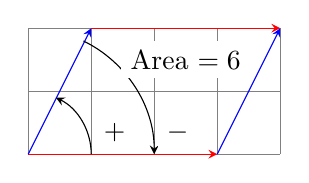
\begin{tikzpicture}[scale=.8]
\draw[help lines,step=1cm] (0,0) grid (4,2);
\draw[->,>=stealth,red] (0,0) -- (3,0);
\draw[->,>=stealth,red] [shift={(1,2)}](0,0) -- (3,0);
\draw[->,>=stealth,blue] (0,0) -- (1,2);
\draw[->,>=stealth,blue] [shift={(3,0)}](0,0) -- (1,2);
\draw[->,>=stealth] (0:1cm)  node[above right=1pt,fill=white]{\normalsize $+$} arc (0:64:1cm) ;
\draw[<-,>=stealth] (0:2cm)  node[above right=1pt,fill=white]{\normalsize $-$} arc (0:64:2cm) ;
\node[fill=white] at (2.5, 1.5) {Area $=6$}; 
\end{tikzpicture}

\vspace{2pt}
$\begin{vmatrix}{3}&{1}\\{0}&{2}\end{vmatrix}=6$ and $\begin{vmatrix}{1}&{3}\\{2}&0\end{vmatrix}=-6$
\end{center}
\caption{The determinant gives both area and direction. A counter clockwise rotation from column 1 to column 2 gives a positive determinant.\label{detfig}}
\end{figure}
%    }}

For a 3 by 3 matrix, the columns give the edges of a three dimensional parallelepiped and the determinant produces the volume of this object. The sign of the determinant is related to orientation. If you can use your right hand and place your index finger on the first vector, middle finger on the second vector, and thumb on the third vector, then the determinant is positive. 
For example, consider the matrix $A = \begin{bmatrix}\cl{1\\0\\0}&\cl{0\\2\\0}&\cl{0\\0\\3}\end{bmatrix}$.  Starting from the origin, each column represents an edge of the rectangular box 
$0\leq x\leq 1$, 
$0\leq y\leq 2$, 
$0\leq z\leq 3$ with volume (and determinant) $V=lwh=(1)(2)(3)=6$. The sign of the determinant is positive because if you place your index finger pointing in the direction (1,0,0) and your middle finger in the direction (0,2,0), then your thumb points upwards in the direction (0,0,3). 
If you interchange two of the columns, for example 
$B = \begin{bmatrix} \cl{0\\2\\0}&\cl{1\\0\\0}&\cl{0\\0\\3}\end{bmatrix}$, then the volume doesn't change since the shape is still the same. However, the sign of the determinant is negative because if you point your index finger in the direction (0,2,0) and your middle finger in the direction (1,0,0), then your thumb points down in the direction (0,0,-3). If you repeat this with your left hand instead of right hand, then your thumb points up.

\begin{problem}
\begin{itemize}
\item Use determinants to find the area of the triangle with vertices $(0,0)$, $(-2,5)$, and $(3,4)$.
\item What would you change if you wanted to find the area of the triangle with vertices $(-3,1)$, $(-2,5)$, and $(3,4)$? Find this area.
\end{itemize}
\end{problem}


\section{Solving Systems of equations}


\begin{problem}
\marginpar{For additional practice, make up your own systems of equations. Use Wolfram Alpha to check your work.}
Solve the following linear system of equations.
\begin{itemize}
\item $\begin{cases}x+y&=3\\2x-y&=4\end{cases}$
\item $\begin{cases}-x + 4y&=8\\3x - 12y&=2\end{cases}$
\end{itemize}
\end{problem}

\begin{problem}
\marginpar{This 
\href{http://www.wolframalpha.com/input/?i=Solve+x\%2B2y\%3D3+and+4x-y\%2Bz\%3D7+and+x\%3Dt}{link} 
will show you how to specify which variable is $t$ when using Wolfram Alpha.}
You main goal is to solve the linear system 
$\begin{cases}x+y+z&=3\\2x-y&=4\end{cases}$.  
You'll notice there are more variables than equations. This suggests there is probably not just one solution, but perhaps infinitely many.  One common way to deal with solving such a system is to let one variable equal $t$, and then solve for the other variables in terms of $t$. Do this three different ways.
\begin{itemize}
\item If you let $x=t$, what are $y$ and $z$.  Write your solution in the form $(x,y,z)$ where you replace $x$, $y$, and $z$ with what they are in terms of $t$.
\item If you let $y=t$, what are $x$ and $z$.
\item If you let $z=t$, what are $x$ and $y$.
\end{itemize}
\end{problem}


\section{Higher Order Approximations} 
When you ask a calculator to tell you what $e^{.1}$ means, your calculator uses an extension of differentials to give you an approximation.  The calculator only uses polynomials (multiplication and addition) to give you an answer.  This same process is used to evaluate any function that is not a polynomial (so trig functions, square roots, inverse trig functions, logarithms, etc.) 
The key idea needed to approximate functions is illustrated by the next problem.

\begin{problem} 
Let $f(x)=e^x$. You should find that your work on each step can be reused to do the next step.
\begin{itemize}
\item Find a first degree polynomial $P_1(x)=a+bx$ so that $P(0)=f(0)$ and $P'(0)=f'(0)$. In other words, give me a line that passes through the same point and has the same slope as $f(x)=e^x$ does at $x=0$. Set up a system of equations and then find the unknowns $a$ and $b$. The next two are very similar.
\item Find a second degree polynomial $P_2(x)=a+bx+cx^2$ so that $P(0)=f(0)$, $P'(0)=f'(0)$, and $P''(0)=f''(0)$. In other words, give me a parabola that passes through the same point, has the same slope, and has the same concavity as $f(x)=e^x$ does at $x=0$. 
\item Find a third degree polynomial $P_3(x)=a+bx+cx^2+dx^3$ so that $P(0)=f(0)$, $P'(0)=f'(0)$, $P''(0)=f''(0)$, and $P'''(0)=f'''(0)$. In other words, give me a cubic that passes through the same point, has the same slope, and has the same concavity as $f(x)=e^x$ does at $x=0$. 
\item Now compute $e^{.1}$ with a calculator.  Then compute $P_1(.1)$, $P_2(.1)$, and $P_3(.1)$. How accurate are the line, parabola, and cubic in approximating $e^{.1}$?
\end{itemize}
\end{problem} 

The previous problem showed you how to create what we call a Taylor polynomial expanded about $c=0$. You showed that the third degree Taylor polynomial expanded about $c=0$ is \marginpar{The factorial function $n!$ for a natural number $n$ is defined  as the product of all the integers upto and including $n$, namely $n!=1\cdot 2\cdot 3 \cdots n$. We define $0!=1$.}
$$P_3(x) = f(0)+\frac{f'(0)}{1!}x+\frac{f''(0)}{2!}x^2+\frac{f''(0)}{3!}x^3. $$  
A similar computation shows that the $n$th degree Taylor polynomial expanded about $c=0$ is
$$P_n(x) = f(0)+\frac{f'(0)}{1!}x+\frac{f''(0)}{2!}x^2+\cdots +\frac{f^{(n)}(0)}{n!}x^n = \sum_{k=0}^n \frac{f^{(k)}(0)}{k!}x^k, $$
where $f^{(k)}$ is the $k$th derivative. To expand about $c=a$, the polynomial is 
$$P_n(x) = f(a)+\frac{f'(a)}{1!}(x-a)+\cdots +\frac{f^{(n)}(a)}{n!}(x-a)^n = \sum_{k=0}^n \frac{f^{(k)}(a)}{k!}(x-a)^k. $$ 
All you do is evaluate each derivative at $a$ instead of $0$, and then replace $x$ with $(x-a)$ to shift everything right $a$. 

\begin{problem}
Let $f(x)=\sqrt{x}$.  Compute the degree 3 Taylor polynomial $P_3(x)$ of $f(x)$ expanded about $c=1$. Then compute $\sqrt{1.2}$ and $P_3(1.2)$.  What is the difference $P_3(1.2)-f(1.2)$? 
You will have found a small change in $y$ (remember we called this $dy$) when the change in $x$ is .2 (so $dx=.2$ since 1.2 is only .2 units away from where we centered out polynomial at $c=1$).
\end{problem}

The problem above introduced the final idea. We will let $dx=x-c$ (a small change in $x$). Since the polynomial should be close to the function, a small change in $y$ is $dy=P_n(x)-f(c)$. We can write the Taylor polynomial notation above in the form  
$$P_n(x) - f(c)=dy=\frac{f'(c)}{1!}dx+\frac{f''(c)}{2!}dx^2+\cdots +\frac{f^{(n)}(c)}{n!}dx^n. $$
If we want to estimate the change in $y$ using a first order approximation, this gives us the differential notation
$$dy = f'(c)dx.$$
A second order approximation is
$$dy = f'(c)dx + \frac{f''(c)}{2!}dx^2.$$
A third order approximation is
$$dy = f'(c)dx + \frac{f''(c)}{2!}dx^2+  \frac{f'''(c)}{3!}dx^3.$$

\begin{example}
This example refers back to problem \ref{diff-sphere}. We want a spherical tank of radius 3m. Let's use a first, second, and third order approximation to estimate how much the volume will increase if the radius is 3.02m instead of 3m.  

We start with $V=4/3 \pi r^3, V'=4\pi r^2, V''=8\pi r,$ and $V'''=8\pi$. Evaluate each of these at $c=3$ to get $V(3)=36\pi, V'(3)=36\pi, V''(3)=24\pi,$ and $V'''(3)=8\pi$. Note that $dx=.02$ as $3.02-3=.02$.
\begin{enumerate}
\item A first order approximation is $$dy=V'(3)dx = 36\pi\cdot .02 = .72\pi.$$
\item A second order approximation is $$dy=V'(3)dx+V''(3)/2!\ dx^2  = 36\pi\cdot .02 +24\pi/2 (.02)^2 =(.7248)\pi.$$
\item A third order approximation is $$dy=V'(3)dx+V''(3)/2!\ dx^2 +V'''(3)/3!\ dx^3  = 36\pi\cdot .02 +24\pi/2 (.02)^2+8\pi/6\ dx^3  =(.724810\bar6)\pi.$$
\end{enumerate}
As a side note, the volume of a sphere involves a cubic function. This means that if we try to approximate the volume with a cubic, we should get an exact approximation.  Use a calculator to check that $$V(3.02)-V(3) = \frac 43 \pi (3.02)^3 - \frac 43 \pi (3)^3 =  (.724810\bar6)\pi.$$ This is precisely what we obtained using our third degree approximation.
\end{example}

We'll end this section with a problem to practice what we did above.

\begin{problem}
Suppose you are constructing a cube whose side length should be $s=2$ units. The manufacturing process is not exact, but instead creates a cube with side lengths $s=2+ds$ units. (You should assume that all sides are still the same, so any error on one side is replicated on all.  We have to assume this for now, but before the semester ends we'll be able to do this with high dimensional calculus.) 

Suppose that the machine creates a cube with side length $2.3$ units instead of 2 units.  Note that the volume of the cube is $V=s^3$.  Use a first, second, and third order approximation to estimate the increase in volume caused by the .3 increase in side length.  Then compute the actual increase in volume $V(2.3)-V(2)$.   
\end{problem}




%%% Local Variables: 
%%% mode: latex
%%% TeX-master: "215-problems"
%%% End: 
